\section{Design}\label{design}


\subsection{Approach}

Our approach is centered around \priceclass{}es. \Priceclass{}es are a metric
that has a number of benefits over resource reservations as an interface:
developers are more likely to have a good sense of it ahead of time, it is less
likely to be different across different invocations, it still gives the
scheduler the information it needs to decide what to schedule when, and finally
it more directly aligns the interests of the developer with those of the
provider by communicating on the level of what the provider and developer
actually care about: money, and latency (as achieved by \class{}es in the
system).


However, having \priceclass{}es also means that there are no clear guarantees
about what they are getting when a developer puts a price on a function they
want to run. In order to mitigate that somewhat and not go into bidding wars, we
propose exposing a fixed set of price classes. This is similar to how AWS has
different EC2 instance types, that are directly mapped to prices. Rather than
being a guarantee, the price class is instead a metric to express priority to
\sys{}, which it can then use to enforce a favoring of high class jobs.



\subsection{Interface}


Developers using \sys{} write function handlers and define triggers just like
they would for any existing serverless offering. In addition, they asign each
function to a price class, this is done at function creation. For instance, a
simple web server might consist of a home page view that is assigned a higher
\priceclass{} and costs 2$\mu\cent$ per cpu second, a user profile page view
which is assigned a middle-high \class{} and cost 1.5$\mu\cent$ per cpu second,
and finally an image processing job that can be set to a low \class{} which
costs only 0.5$\mu\cent$ per cpu second.

\Class{}es are inherited across call chains: if a high \class{} job calls a low
\class{} job, that invocation with run with high \class{}. This is important in
order to avoid priority inversion.

Developers pay for memory separately, and by use; the price for memory is the
same across all \class{}es.

To avoid unexpected costs in the case of for example a DOS attack or a bug,
developers also express a monthly budget that they are willing to pay.\ \sys{}
uses this budget as a guideline and throttles invocations or decreases quality
of service in the case that usage is not within reason given the expected
budget, though it does not guarantee that the budget will not be exceeded by
small amounts.



\subsection{\Sys{} Design}

\begin{figure}[t]
    \centering
      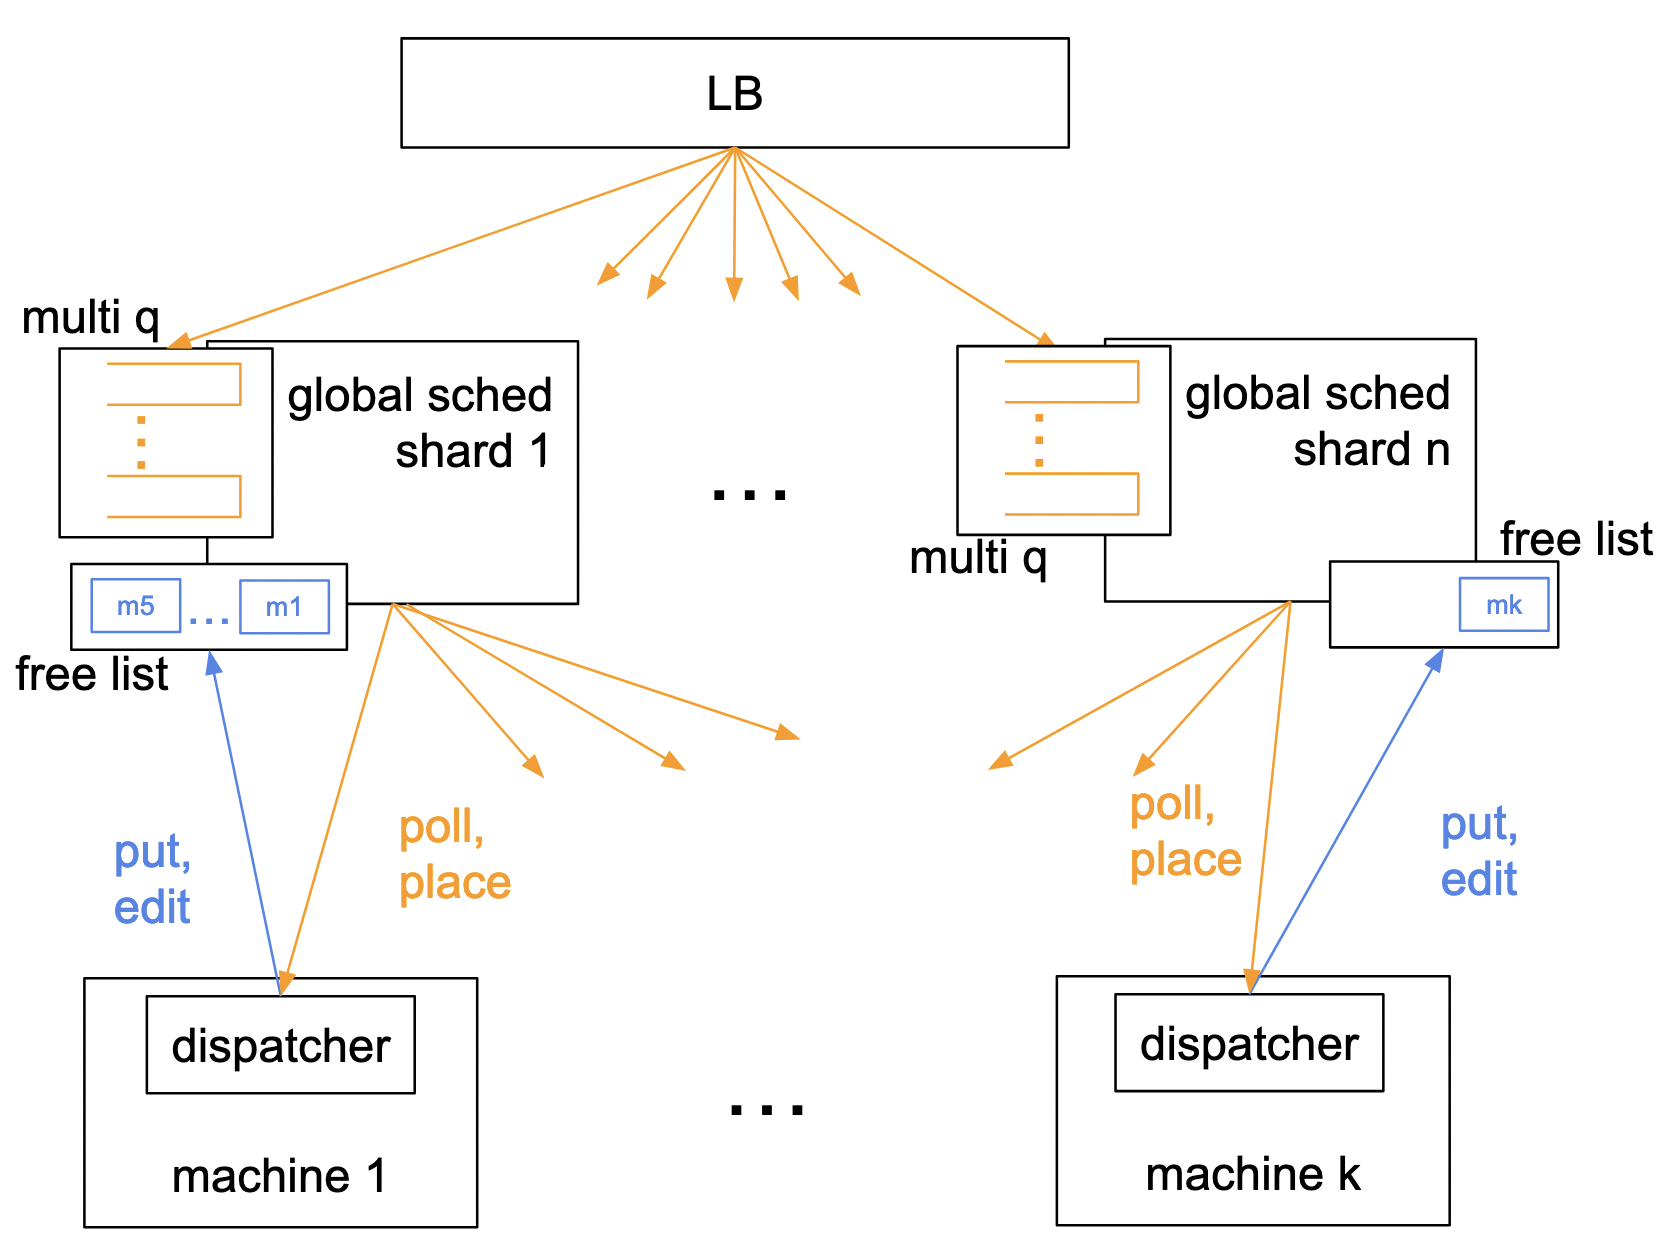
\includegraphics[width=9cm]{img/overview.png}
      \caption{ global scheduler shards queue and place jobs (in orange), 
      on each machine a dispatcher thread keeps track of memory utilization 
      and if it's low writes itself to an idle list (in blue) }
    \label{fig:overview}
\end{figure}



\Sys{} has as its goal to enforce the \class{}es attached to jobs, which means
it needs to prefer higher \class{} jobs over lower ones, and preempt the latter
when necessary.
  

As shown in Figure~\ref{fig:overview}, \sys{} sits behind a load balancer, and
consists of: a \textit{distributed global scheduler}, which places new job
invocations and has attached an \textit{idle list}, a \textit{dispatcher},
which runs on each machine and communicates with the global scheduler shards,
and a \textit{machine scheduler}, which enforces \class{}es on the machines.


\textbf{Machine Scheduler.}
The machine scheduler is a preemptive priority scheduler: it preempts lower
\class{} jobs to run higher \class{} ones. Being unfair and starving low
\class{} jobs is desirable in \sys{}, since image processing jobs should not
interrupt a page view request processing, but vice versa is expected. Within
\class{}es the machine scheduler is first come first served. This matches Linux'
`sched fifo' scheduling.
% https://man7.org/linux/man-pages/man7/sched.7.html


\textbf{Idle list.}
Each global scheduler shard has an idle list, which holds machines that
have a significant amount of memory available. In the shards idle list each
machine's entry is associated with the amount of free memory as well as the
current amount of jobs on the machine. The idle list exists because datacenters
are large: polling a small number of machines has been shown to be very
powerful, but cannot find something that is a very rare occurrence.
% join idle queue
What this means is that polling is likely to find a machine in the lower
quantile of the datacenter, but not at the absolute bottom --- it will not find
one of the handful of machines that are actually idle. Having an idle list
allows these machines, which are expected to be rare in a high-utilization
setting, to make themselves visible to the global scheduler. The idle list also
allows the global scheduler to place high \class{} processes quickly, without
incurring the latency overheads of doing the polling to find available
resources.


\textbf{Dispatcher.}
The dispatcher is in charge of adding itself to a shard's idle list when memory
utilization is low. The dispatcher chooses which list to add itself to using
power-of-k-choices: it looks at k shards' idle lists and chooses the one with
the least other machines in it. If the machine is already on an idle list on
shard $i$, but the amount of available memory has changed significantly (either
by jobs finishing and memory being freed or by memory utilization increasing
because of new jobs or memory antagonists), the dispatcher will update shard
$i$'s idle list. These interactions from the dispatcher to free lists are
represented by the blue arrows in Figure~\ref{fig:overview}.

The dispatcher is also in charge of managing the machine's memory. When memory
pressure occurs, the dispatcher uses \textit{\class{}-based swapping} to move low
\class{} processes off the machine's memory. In this scenario, having priority
scheduling creates the opportunity that enables this to be realistic: because
the dispatcher knows that the lowest \class{} jobs will not be run until the
high \class{} jobs have all finished, it can swap its memory out knowing it will
not be needed soon. Avoiding a churn of jobs with swapped memory that are being
swapped in and out as they are scheduled in and out, requires that the memory of
the machine is large against the amount of memory that could be used by as many
jobs as the machine has cores. This assumption ensures that memory pressure high
enough to require swapping will only occur when there are many more jobs than
there are cores, and thus that the swapped job will not be running soon. The
dispatcher swaps the low \class{} job back in when the memory pressure is gone
and the job will be run.

% \makeatletter
% \renewcommand{\ALG@name}{Procedure}
% \makeatother
% \begin{algorithm}[t]
% \caption{Choosing a machine for a job j}\label{alg:place}
% \begin{algorithmic}
%     \If{$|idleList| > 0$} \\
%         \Return$ $min(qLen)
%     \EndIf
%     \State$M = $ qlen of k polled machines
%     \If{min(M.timeToProfit$) < THRESH$} \\
%         \Return$ $min($M$)
%     \Else
%         \State$ $reQ j, with priority -= 1
%     \EndIf
% \end{algorithmic}
% \end{algorithm}


\textbf{Global Scheduler Shards.}

Global scheduler shards store the jobs waiting to be placed in a multi queue,
with one queue per \priceclass{}. Shards choose what job to place next by
looking at each job at the head of each queue, and comparing the ratio of
\class{} to amount of time spent in the queue. This ensures that high \class{}
jobs don't have to wait as long as lower \class{} jobs to be chosen next, but
low \class{} jobs will get placed if they have waited for a while.

When placing the chosen job, the shard will first look in its idle list. If the
list is not empty, it will choose the machine with the smallest queue length.

If there are no machines in the idle list, the shard switches over to
power-of-k-choices: it polls k machines, getting the amount of jobs running from
each. The shard then places the new job on the machine with the smallest number
of currently running jobs. It is desirable to have a maximally heterogenous set
of \class{}es on each machine, but since jobs come in randomly the global
scheduler does not explicitly have to enforce this.
